\clearpage
\chapter{Background Estimation}\label{sec:estimate}

Section ~\ref{sec:selections} listed several different discriminant variables for the analysis.
Leading ROI vertex score, subleading ROI vertex score, and leading muon's IP value have the most discriminatory power.
Although the background MC samples describe the data's distribution fairly well, one can also see discrepancy at higher vertex score and higher IPSig values.
This originates from 2 different reasons.
First, the lack of statistics is a fundamental deficiency for the MC samples.
Unlike 11.9 billion events b-parking data, MC sample events are simulated with extremely intensive computing resources.
Thus, its event number is limited below 100 milion at most, failing to describe distributions for extreme values.
Second, the QCD MC's data description accuracy lacks compared to other physics process.
QCD background, which is the main background for the analysis, is a quantum-chromodynamics process.
QCD involves a lot of uncertainty and relies on probablistic description at low energy.
Therefore, QCD's description accuracy lacks compared to other process such as WJets and Drell-Yan process.
Since MC does not describe the data in a satisfactory manner, the analysis uses data-driven background estimation method.


\section{ABCD method}
For any background estimation method, ABCD method is the most preferred thanks to its simplicity.
ABCD method is a simplest form of transfer-factor.
A ratio of background event at 2 control region (CR) is applied to another CR's background event to infer background event in signal region (SR) without unblinding.
Simplest mathematical for is described in formula \ref{eq:ABCD}.
\begin{equation}
\label{eq:ABCD}
	SR:CR1=CR2:CR3, SR=CR1*\frac{CR2}{CR3} 
\end{equation}
ABCD method requires 2 variables used for its estimation should be independent of each other for background process.


Unfortunately, leading ROI vertex score and subleading ROI vertex score are correlated in the QCD background process.
ROIs from B-mesons score higher in our tensorflow.
In QCD processes, the B-mesons are likely to be pair produced.
Therefore, when the leading ROI vertex score is high due to its b-like behavior, the sublead ROI vertex score is also high because the anti-meson is produced on the other side of the detector.
Thus, leading and sublead scores can't be our ABCD discriminant variable candidates du to their correlation.

The analysis selects leading ROI and leading muon's IP value as its ABCD discriminant variables.
After implementing all other cuts (sublead ROI, $\Delta\Phi(lead,sublead)$, Annulus score, 1 Isolated $\mu$, $\Delta R(lead ROI, Jet)$), we tested the correlation factor between the leading ROI, and leading mu's IPSig values for each background process.
The values are pretty minimal except for 2-3 processes where there were too few entries to derive a physical conclusion due to statistical limitations.
Therefore, the analysis uses leading Log10(IPSig) and leading ROI vertex score for its ABCD discriminant variables.

The results are listed below.  


 \begin{figure}[h!]
   \caption{Cutflow histogram of MS15GeV-ct100mm point. Left plot is for region A, whereas the right plot is for region D}
   \label{fig:ABmethod}
   \centering
   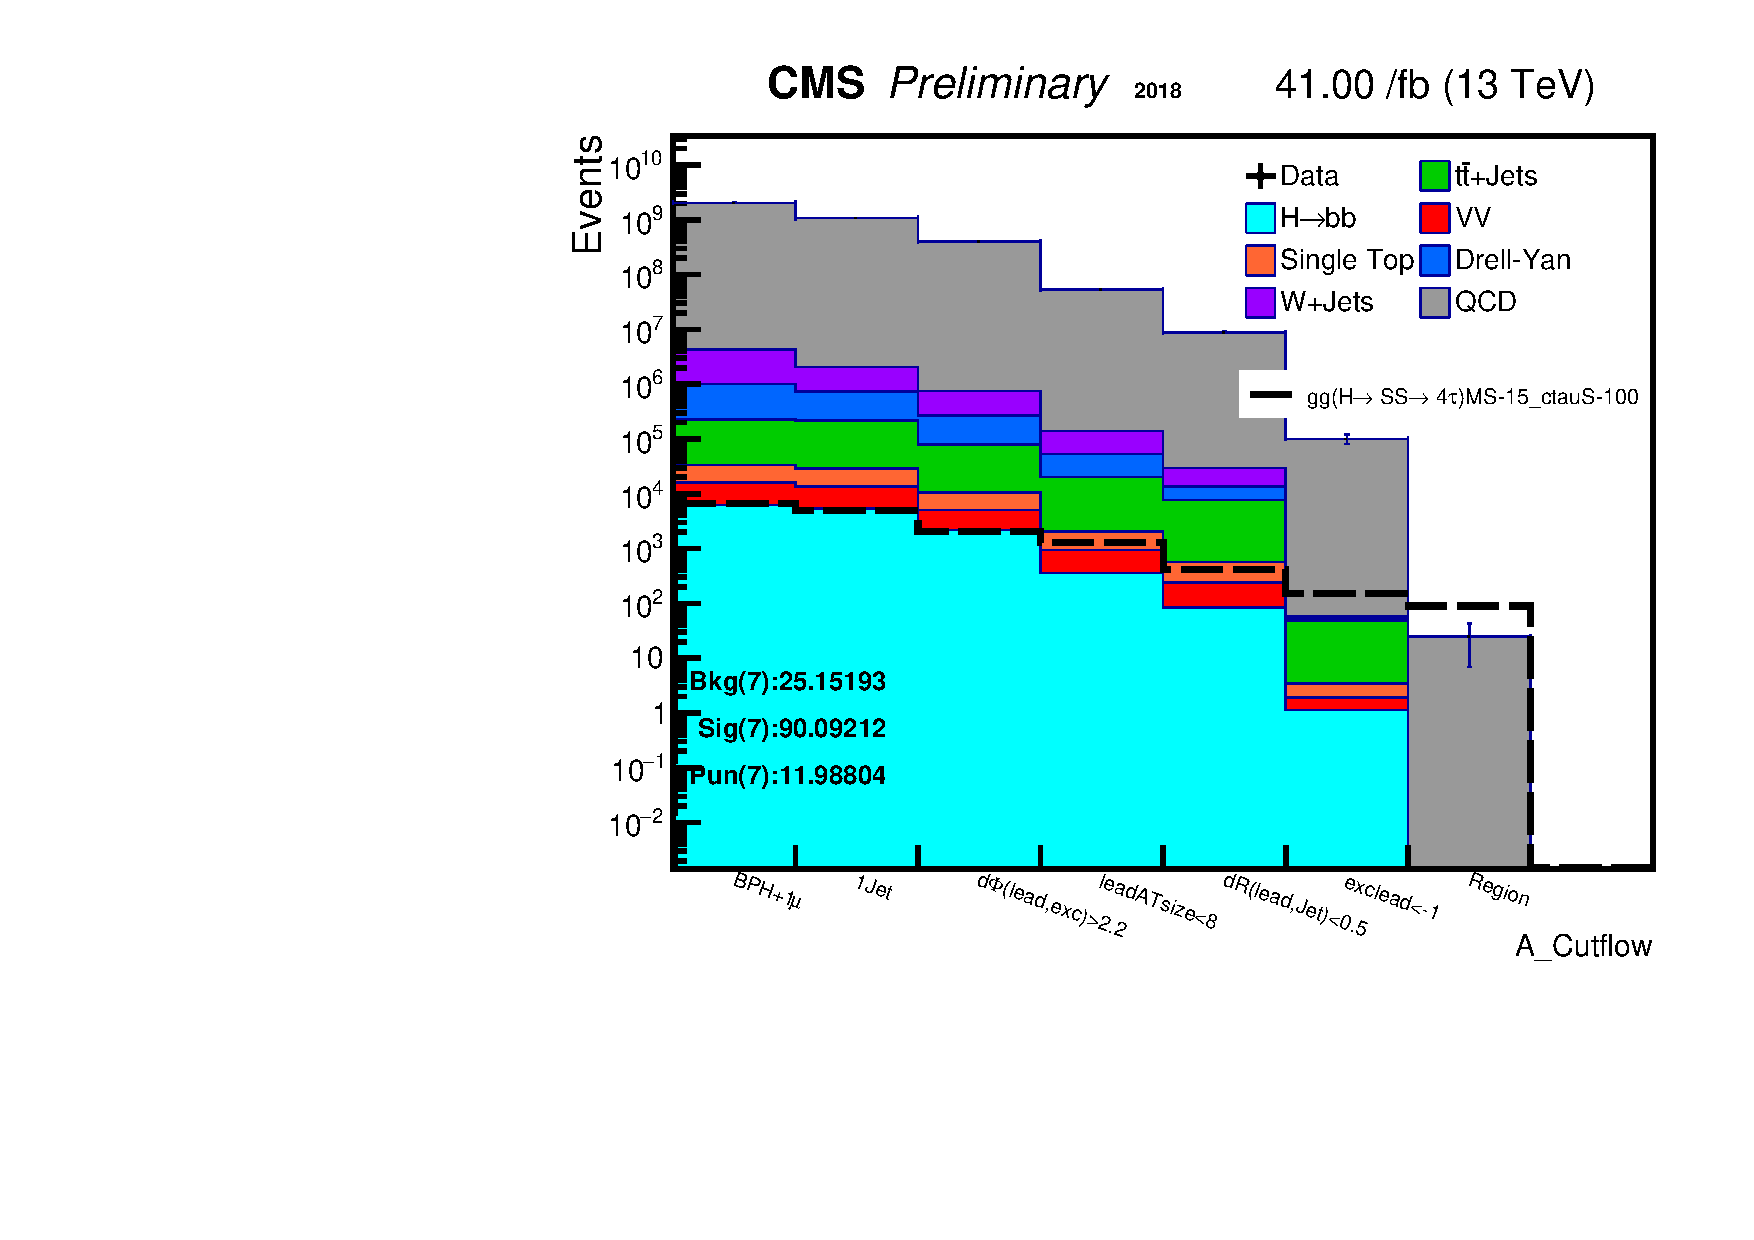
\includegraphics[width=0.47\linewidth]{figs/AnalysisNoteplot_MS-15_ctauS-100_A_Cutflow.pdf}
   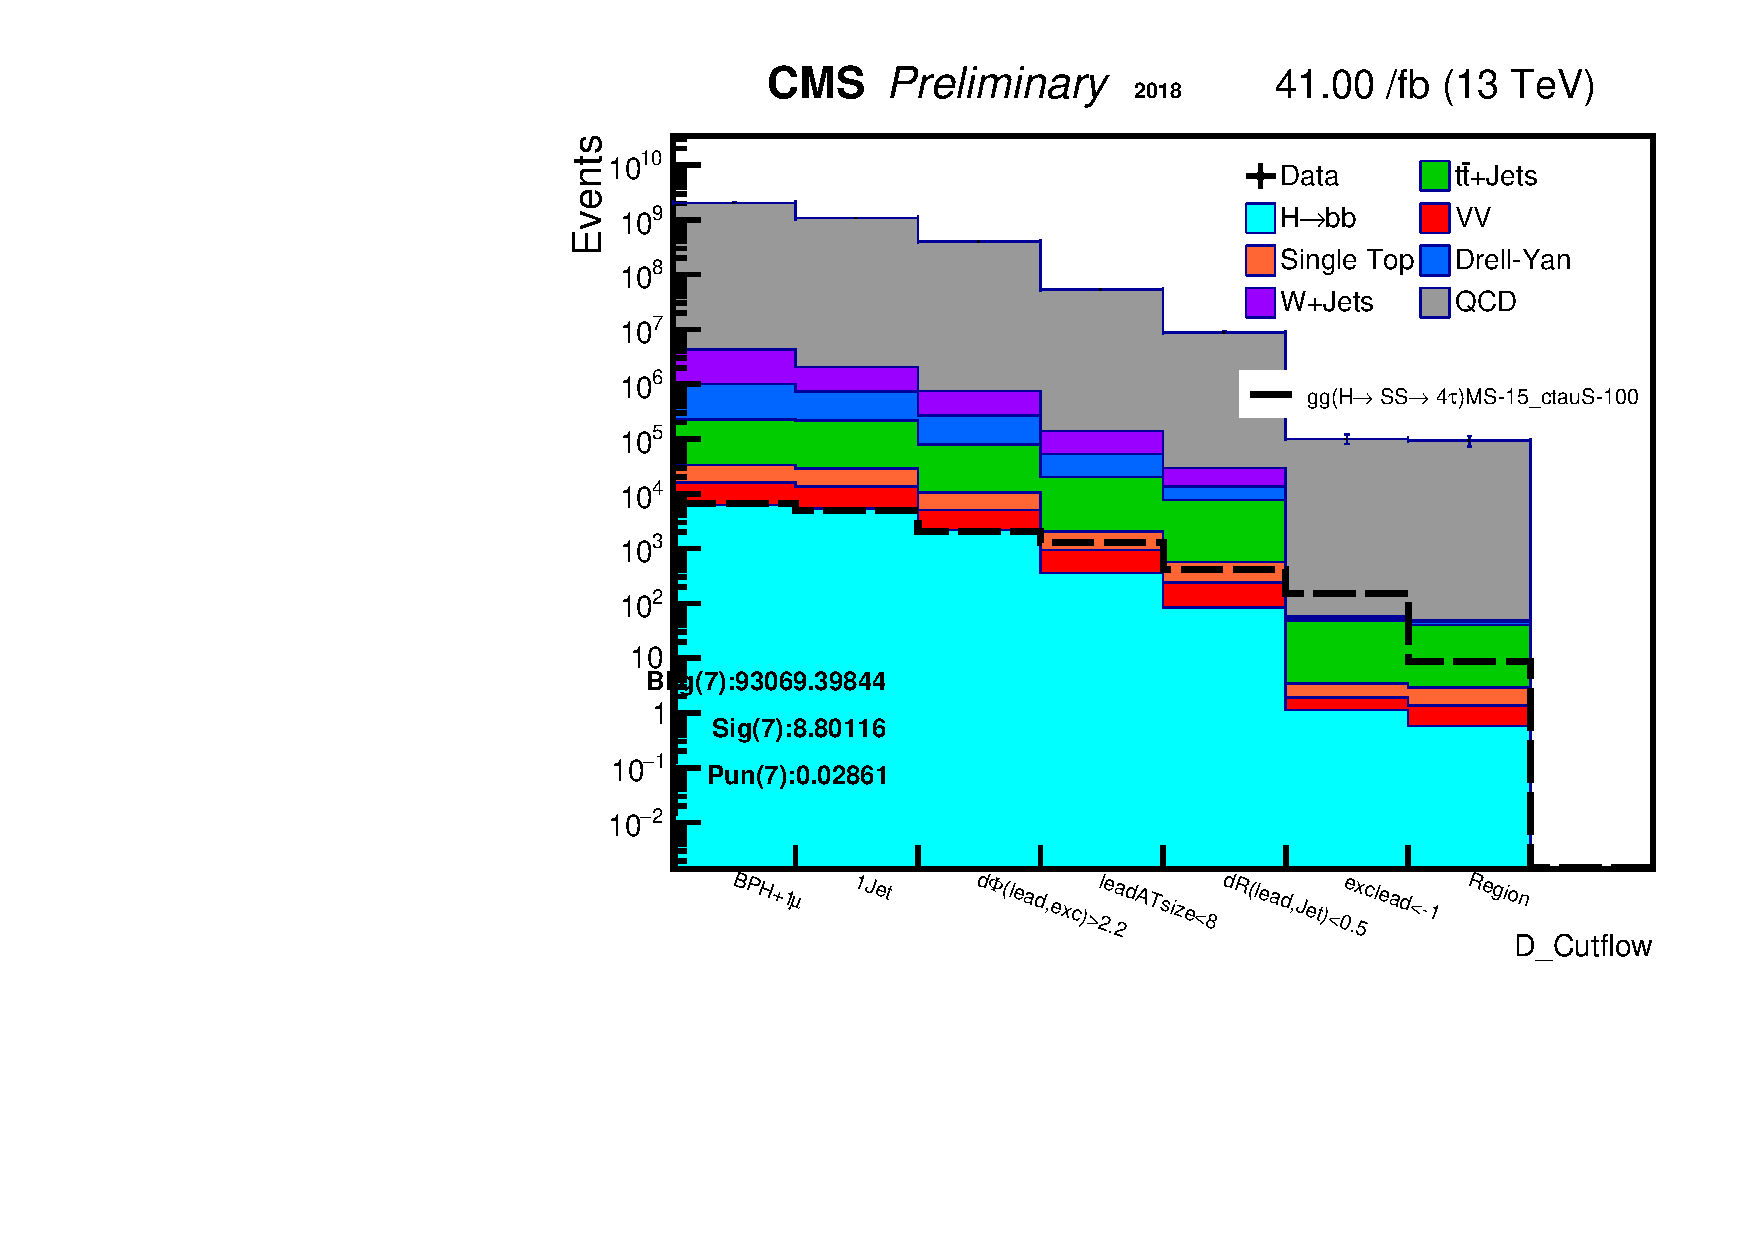
\includegraphics[width=0.47\linewidth]{figs/AnalysisNoteplot_MS-15_ctauS-100_D_Cutflow.pdf}
 \end{figure}

 \begin{figure}[h!]
   \caption{eee}
   \label{fig:ABCDmethod}
   \centering
   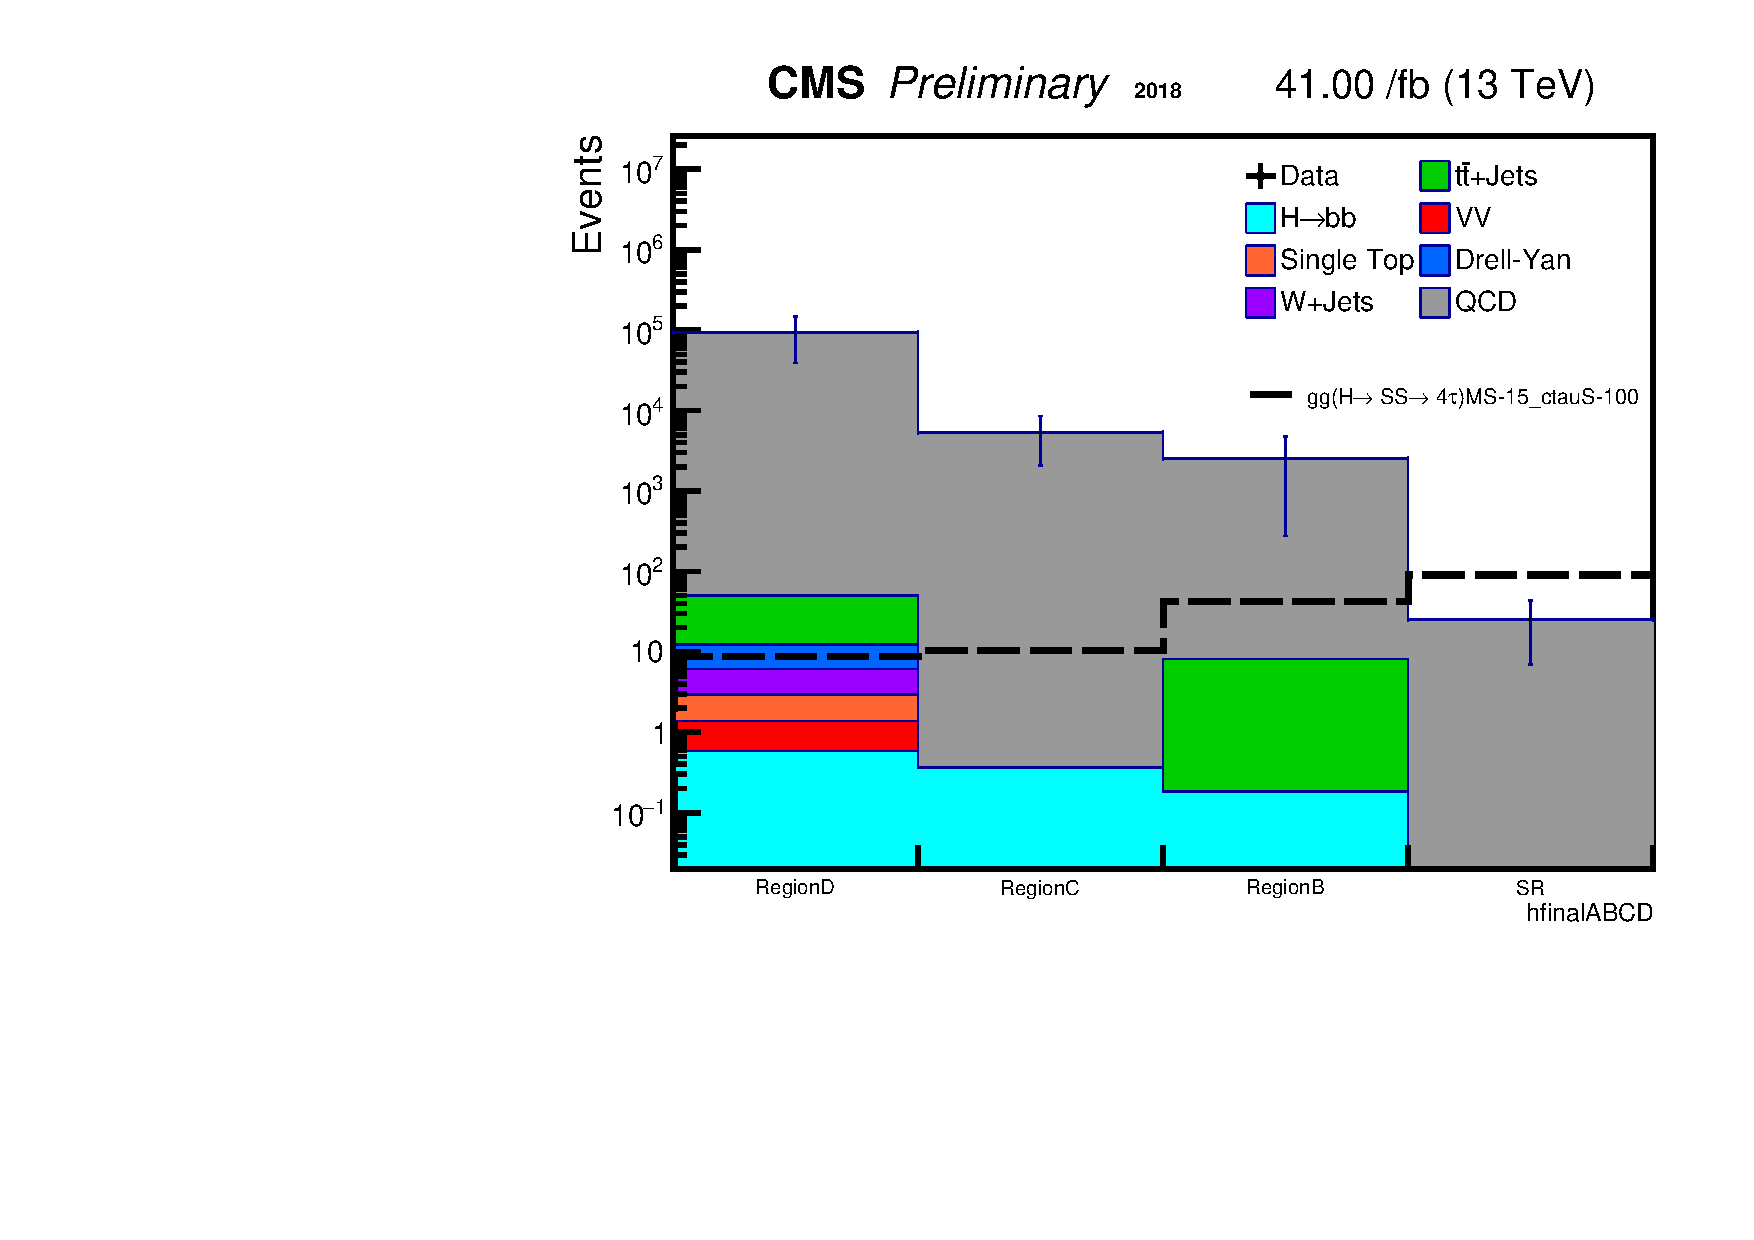
\includegraphics[width=0.67\linewidth]{figs/AnalysisNoteplot_MS-15_ctauS-100_hfinalABCD.pdf}
 \end{figure}

 \section{Validation of ABCD method}


